\chapter{Document Planning}
\label{cap:document_planning}

En la arquitectura presentada en el capítulo~\ref{cap:nlg_intro} mencionamos que el \emph{document planner} es el responsable de decidir que información comunicar (\emph{determinación de contenido}) y como deberá estar estructurada esta información en el texto final (\emph{estructuración de documento}). El document planner será el encargado de que el documento final contenga toda la información requerida por el usuario y que la misma se encuentre estructurada de una forma razonablemente coherente. El resultado de esta etapa será un \emph{document plan} en el cual se especifica qué contenido debe ser incluido en el texto final y de que forma debe estar estructurado.


A continuación describiremos brevemente la entrada y salida de nuestro \emph{document planner}, definiremos como modelar los elementos informativos (estos serán elementos de nuestro \emph{document plan}) y finalmente describiremos las tareas de \emph{determinación de contenido} y \emph{estructuración de documento}.

\section{Entrada y salida del document planner}
Como el document planner es el primer módulo del pipeline, la entrada del document planner será la misma que la entrada de nuestro sistema. Reiter y Dale~\cite{reiter_dale} generalizan la entrada de un sistema de NLG  como una cuádrupla compuestas por los siguientes componentes:

\bigskip
\noindent
\emph{Fuente de conocimiento:} Se refiere a las bases de datos e información del dominio de aplicación que nos proporcionará el contenido de la información que los textos generados deberán contener.
En nuestro caso la fuente de conocimiento estará compuesta por la especificación, las designaciones de la misma y las clases y casos de prueba generados.

\bigskip
\noindent
\emph{Objetivo comunicacional:} Especifica el propósito que debe cumplir el sistema. En general esta compuesto por un ``tipo de objetivo'' y un parámetro.
En este trabajo tendremos solo un tipo de objetivo comunicacional: \emph{Describir(x)}, dónde el parámetro \emph{x} será un conjunto de identificadores de las clases de prueba que desean describirse.

\bigskip
\noindent
\emph{Modelo de usuario:} Provee información acerca del usuario (nivel de experiencia, preferencias, etc.). En nuestro caso el sistema se comportará de la misma forma independientemente del usuario, por lo que no tendremos en cuenta información del mismo.

\bigskip
\noindent
\emph{Historial de discurso:} Consta de información sobre interacciones previas entre el usuario y el sistema. Este historial puede servir para algunos sistemas interactivos donde las interacciones previas con el usuario pueden resultar de utilidad. 

\bigskip
La salida del document planner será un document plan. En nuestra arquitectura el document plan está estructurado como un árbol, donde las hojas representan el contenido y los nodos internos especifican información estructural, por ejemplo sobre como debe agruparse la el contenido a comunicar. En la sección~\ref{sec:document_structure} desarrollaremos este tema mas en detalle.

\section{Representación del dominio}

En los sistemas de NLG el texto generado se utiliza principalmente para transmitir información. Esta información será expresada generalmente en frases y palabras, pero estas  frases y palabras no son en si mismo la información; la información subyace estos constructores lingüísticos y es ``llevada'' por ellos. Nos deberemos concentrar entonces en como representar este conocimiento y como ``mapear'' estas estructuras a una representación semántica. 


El \emph{corpus de descripciones} (apéndice~\ref{sec:apendice1}) resulta una buena fuente para estudiar y definir como deberemos representar la información o \emph{mensajes}\footnote{Reiter y Dale llaman \emph{mensajes} a elementos informativos que conceptualizan la información que queremos comunicar. Estos están compuesto en sí mismos por elementos del dominio de aplicación.} a comunicar. Podemos ver en todos los ejemplos del \emph{corpus} una relación directa entre la información a comunicar y las expresiones Z pertenecientes al dominio de aplicación, donde podemos observar que cada linea de una descripción se corresponde perfectamente con la verbalización de la expresión en lenguaje Z correspondiente. Veamos por ejemplo las siguientes líneas de la descripción de LookUp\_SP\_1 introducida anteriormente (pág.~\pageref{fig:ej_desc_lookup_sp_1}):

\medskip
\begin{enumerate}
 \item{\emph{``El símbolo a buscar pertenece a los símbolos cargados en la tabla de símbolos.''}}
 \item{\emph{``El símbolo a buscar es el único elemento del conjunto formado por los símbolos cargados en la tabla de símbolos.''}}
\end{enumerate}

\medskip
\noindent
en las que podemos observar que la información de cada linea de la descripción se encuentra perfectamente caracterizada por la expresión Z que describe, enumeradas a continuación:

\medskip
\begin{enumerate}
  \item{$s? \in \dom st$}
  \item{$\dom st = \{ s? \}$}
\end{enumerate}

%TODO faltaria hablar un poco de las designaciones, no se ve que sea tan sencilla como se dice esta caracterizacion

\medskip
Debido a esta correlación entre las expresiones de las clases de prueba y la información a generar, la verbalización de las mismas, podemos establecer un único tipo de \emph{mensaje} para nuestro sistema: \emph{VerbalizacionExpresion}. Este representa, como su nombre lo indica, una verbalización de una expresión Z. En la figura~\ref{fig:ej_mensajes} podemos ver como quedarían definidos los mensajes para las dos lineas de la descripción de \emph{LookUp\_SP\_1} vista anteriormente.

\begin{figure}[H]
  	\centering
	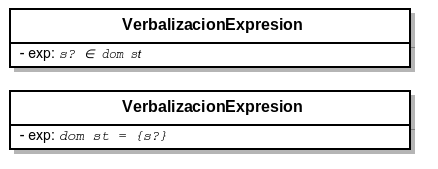
\includegraphics[scale=0.4]{img/mensajes.png}
	\caption{Mensajes a comunicar para el ejemplo de la figura~\ref{fig:ej_desc_lookup_sp_1}.}
  	\label{fig:ej_mensajes}
\end{figure}



\section{Determinación del contenido}

La determinación del contenido es el nombre que se le da a la tarea de decidir y obtener la información que se debe comunicar en un texto. Este proceso generalmente involucra una o más tareas de selección, resumen y razonamiento con los datos de entrada.
El \emph{proceso de selección} recopilará un subconjunto de la información de entrada para luego poder ser comunicada al usuario. El objetivo del mismo será el de proveer la información relevante requerida por el mismo.
La tarea de \emph{resumen} es necesaria cuando los datos de entrada son muy ``granulados'' para ser comunicados directamente o si la información relevante consiste alguna generalización o abstracción de los mismos, que no es el caso de nuestro sistema donde las expresiones de Z con las que trabajaremos contienen exactamente la información que se desea comunicar.
Por último el \emph{razonamiento con los datos} resulta un caso general de las dos anteriores. Finalmente, una vez seleccionada y procesada la información necesaria será esta etapa la encargada de construir los mensajes introducidos en la sección anterior, que luego formarán parte de nuestro \emph{document plan}.
%TODO revisar traduccion de fine-grained -> "granulados"

Para nuestro trabajo, la tarea de selección se resume en la búsqueda y filtrado de las clases de prueba indicadas por el usuario dentro de todo el conjunto de clases de prueba que forma parte de la entrada de nuestro sistema. Por ejemplo, si deseamos generar una descripción para la clase de prueba \emph{LookUp\_SP\_1} de la figura~\ref{fig:ej_tcl_lookup}, la misión de de esta tarea será la de identificar y seleccionar la clase de prueba \emph{LookUp\_SP\_1} entre todas las clases de pruebas que forman parte de los datos de entrada de nuestro sistema de NLG.

Luego de la selección, nuestro sistema deberá procesar los datos de entrada con el fin de obtener mejores descripciones. Hemos observado\footnote{Las observaciones son en base a clases de prueba generados utilizando \emph{Fastest 1.6}} que trabajando ciertas expresiones en las clases de prueba podemos mejorar considerablemente los textos generados. Veamos por ejemplo la figura~\ref{fig:ej_update_sp_4} donde se muestra una clase de prueba generada con \emph{Fastest} en la que se pueden ver dos problemas que abordaremos en esta etapa.

\begin{figure}[H]
  \centering
  \begin{schema}{Update\_ SP\_ 4}\\
   st : SYM \pfun VAL \\
   s? : SYM \\
   v? : VAL 
  \where
   st \neq \{ \} \\
   \{ s? \mapsto v? \} \neq \{ \} \\
   \dom st = \dom \{ s? \mapsto v? \}
  \end{schema}
  \caption{Clase de prueba para operación Update (pág.~\pageref{fig:spec_symbol_table}).}
  \label{fig:ej_update_sp_4}
\end{figure}

Podemos observar que la siguiente expresión del ejemplo anterior:

\begin{figure}[H]
  \centering
  $\{ s? \mapsto v? \} \neq \{ \}$ 
\end{figure}

\noindent
no aporta información importante para el usuario, de hecho esta expresión no agrega ninguna restricción para el caso de prueba ya que será siempre verdadera. De no filtrar esta expresión tempranamente, terminaríamos como resultado un texto generando parecido al siguiente:

\begin{figure}[H]
  \emph{``el conjunto formado por el par de el símbolo a actualizar y el nuevo valor, es distinto al conjunto vacío''}
\end{figure}

\noindent
que además de resultar algo difícil de interpretar, no aporta nada al objetivo comunicacional.

Por otro lado, en un primer intento por describir automáticamente la expresión:

\begin{figure}[H]
  \centering
  $\dom st = \dom \{ s? \mapsto v? \}$ 
\end{figure}

\noindent
podríamos describirla como\footnote{Esta descripción sería la generada utilizando el sistema de reglas propuesto en el capítulo~\ref{TODO} si no trabajamos la expresión en una etapa previa.}:

\begin{figure}[H]
  \emph{``el conjunto de símbolos cargados en la tabla es igual a el dominio del par formado por el símbolo a actualiza y el nuevo valor''}
\end{figure}

Es posible simplificar notablemente esta descripción si antes trabajamos la expresión anterior, que resulta equivalente a:

\begin{figure}[H]
  \centering
  $\dom st = \{s?\}$ 
\end{figure}

\noindent
que luego podríamos describir como:

\begin{figure}[H]
  \emph{``el símbolo a actualizar es el único elemento en la tabla de símbolos cargados''}
\end{figure}

En conclusión, el procesamiento que nos proponemos a realizar en esta etapa tendrá dos objetivos:
\begin{enumerate}
  \item Eliminar tautologías de las expresiones que forman parte de las clases de prueba seleccionadas.
  \item Realizar algunas simplificaciones o reducciones triviales.
\end{enumerate}

\bigskip
Una vez seleccionada y procesada la información deberemos construir los \emph{mensajes} (\emph{VerbalizacionExpresion}) que luego formarán parte del \emph{document plan} desarrollado en el siguiente capítulo.

\section{Estructuración del documento}

Como dijimos antes, el texto generado no podrá ser una colección al azar de frases y palabras. Deberá tener coherencia y poseer una estructura que le permita al lector interpretar con facilidad el contenido del mismo.
Necesitaremos considerar como organizar y estructurar la información que debemos comunicar con el fin de producir un texto razonablemente fácil de leer y comprender.

%~\footnote{Las decisiones sobre como debe estar ordenado y agrupado el documento final son resultado del análisis del \emph{corpus} de descripciones.}
En esta tarea nos concentraremos en construir una estructura que contenga los \emph{mensajes} seleccionados en la etapa de \emph{determinación de contenido}; estableciendo el agrupamiento y ordenamiento de los mismos. Esta estructura deberá caracterizar la disposición de los elementos pertenecientes a los textos recopilados en el \emph{corpus}. 

Tomando el \emph{corpus} de descripciones como una especificación de los documentos que debemos generar podemos observar que estos documentos poseen una estructura bastante simple y rígida a la vez. Estos documentos deben estar formados por una secuencia de descripciones para las clases de prueba indicadas por el usuario, ordenadas alfabéticamente según el nombre de la clase de prueba. A su vez, cada una de estas descripciones deberá agrupar las verbalizaciones de las expresiones seleccionadas en la etapa de \emph{determinación de contenido}, ordenadas de la misma forma en la que aparecen en el esquema de la clase de prueba en cuestión. En la figura~\ref{fig:png_document_plan} podemos observar una representación abstracta de la estructura propuesta para modelar el documento.

\begin{figure}[H]
  	\centering
	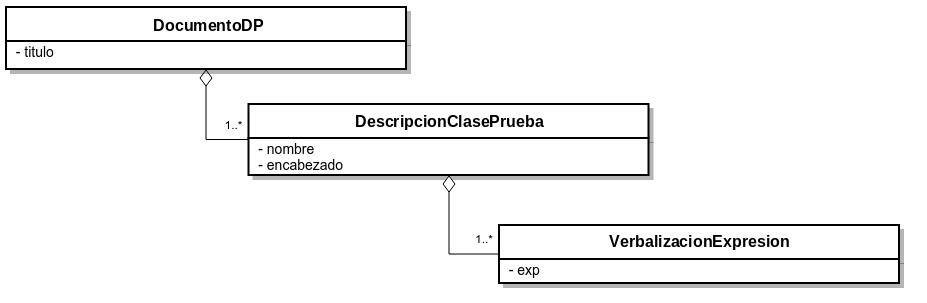
\includegraphics[scale=0.4]{img/document_plan.png}
	\caption{Document plan.}
  	\label{fig:png_document_plan}
\end{figure}

Llamaremos \emph{DocumentoDP} a la raíz de nuestro \emph{document plan}, \emph{DocumentoDP} contendrá a su vez una lista ordenada de las descripciones de las clases de prueba (\emph{DescripcionClasePrueba}) que debemos incluir en el texto final. El elemento \emph{DescripcionClasePrueba} representa el texto a generar para una clase de prueba (por ejemplo el texto de la figura~\ref{fig:ej_lookup_sp_1}) y tendremos uno de estos elementos por cada clase de prueba indicada por el usuario. Finalmente los mensajes seleccionados en la etapa anterior formarán se encontrarán agrupados en la \emph{DescripcionClasePrueba} correspondiente. Podemos ver en la figura~\ref{fig:png_document_plan_ej} un ejemplo del document plan para la descripción de la clase de prueba \emph{LookUp\_SP\_1} introducida anteriormente. 

\begin{figure}[H]
  	\centering
	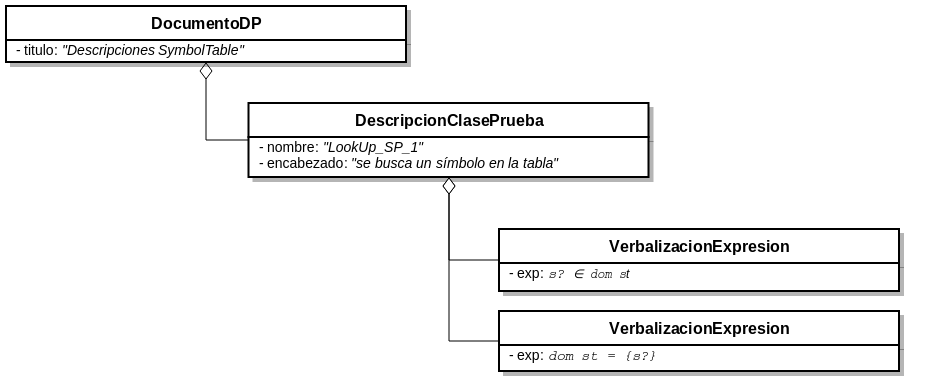
\includegraphics[scale=0.4]{img/document_plan_ej.png}
	\caption{Document plan correspondiente al texto de la figura~\ref{fig:ej_lookup_sp_1}.}
  	\label{fig:png_document_plan_ej}
\end{figure}


\label{sec:document_structure}